\chapter{3D Modelling and Animation}

\section*{3D Modelling}
The 3D model of the da Vinci robot was created in Autodesk 3DS Max. The robot needed to be modelled as realistic as possible and as such the program was chosen based on it's level of detail and built-in functions. However, due to the location and observation limitations of the da Vinci Si System it was not possible to capture every detail of the robot. As such, the robot is modelled partially from images taken, images on the internet, and memory. The robot was modelled with box modelling and was compared to a human model to ensure somewhat realistic sizes of the individual parts. The workspace for 3DS Max is shown in \autoref{Fig:Maximus}

\begin{figure}[H]
	\centering
	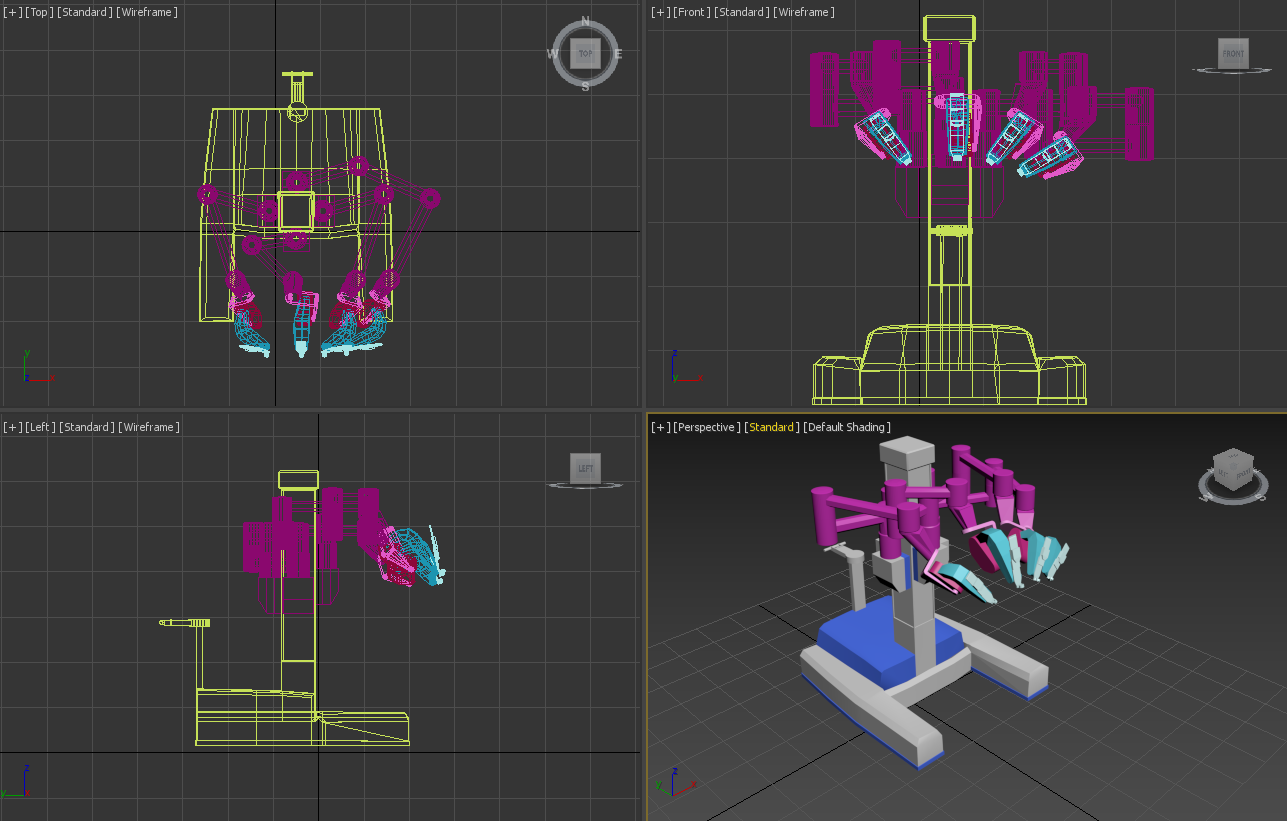
\includegraphics[width=0.75\textwidth]{ModelAnim/Max}
	\caption{The robot shown in Max' default workspace separated into four perspective views}
	\label{Fig:Maximus}
\end{figure}

Upon completion, the model was imported into Autodesk Maya which allows for easier rigging and animation. The model was rigged according to the joints of the real robot. The workspace for Mayas' workspace can be seen in \autoref{fig:mayasimus}

\begin{figure}[H]
	\centering
	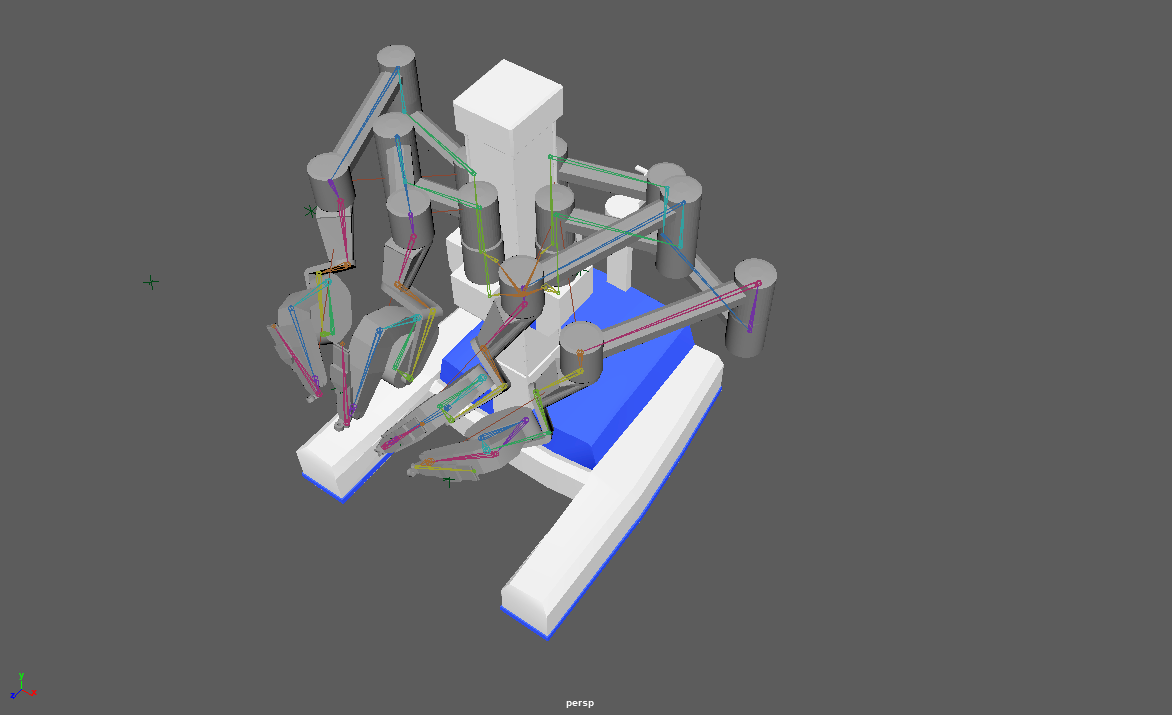
\includegraphics[width=0.75\textwidth]{ModelAnim/RobotMaya}
	\caption{The robot shown in Maya's default workspace indicating bones}
	\label{fig:mayasimus}
\end{figure}

\section*{3D Animation}
A 3D animation was created to ensure that pseudo-realistic docking procedure could procede as a backup for the real-time interaction due to time constraints. In the case of using animation instead of interaction, a button would have to implemented in the scene to start the animation. This animation could then be reversed to simulate undocking.

\begin{figure}[hpbt]
	\centering
	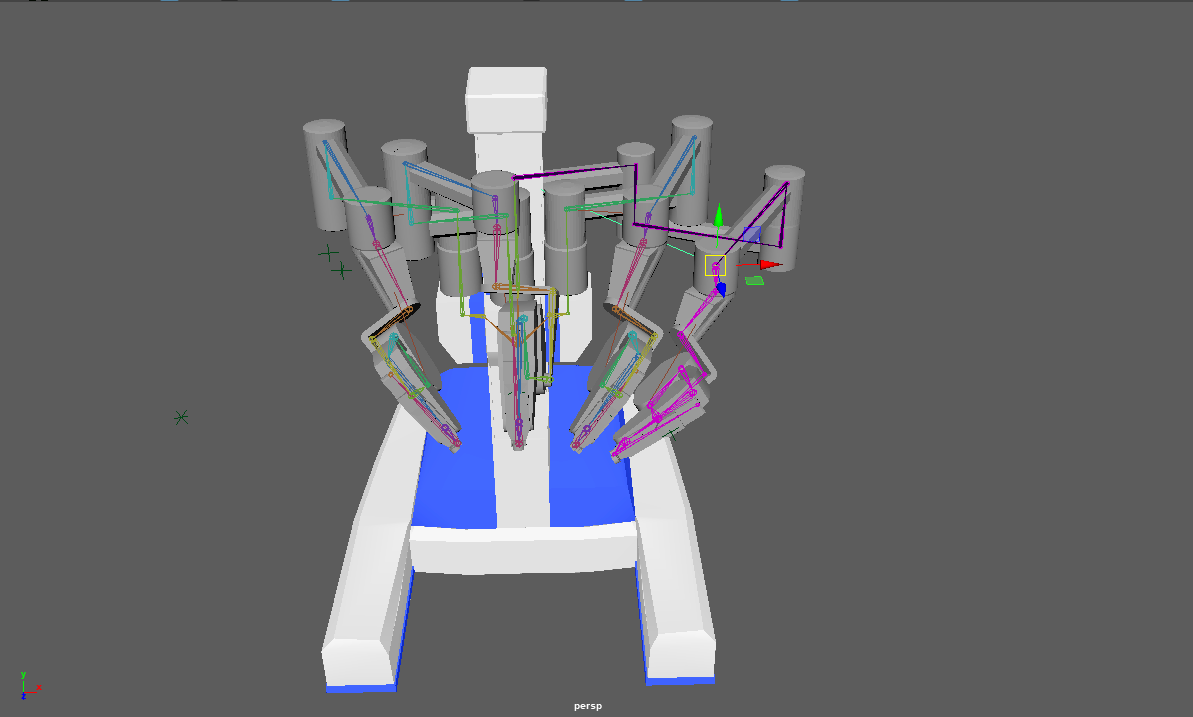
\includegraphics[width=0.3\textwidth]{ModelAnim/IK1}
	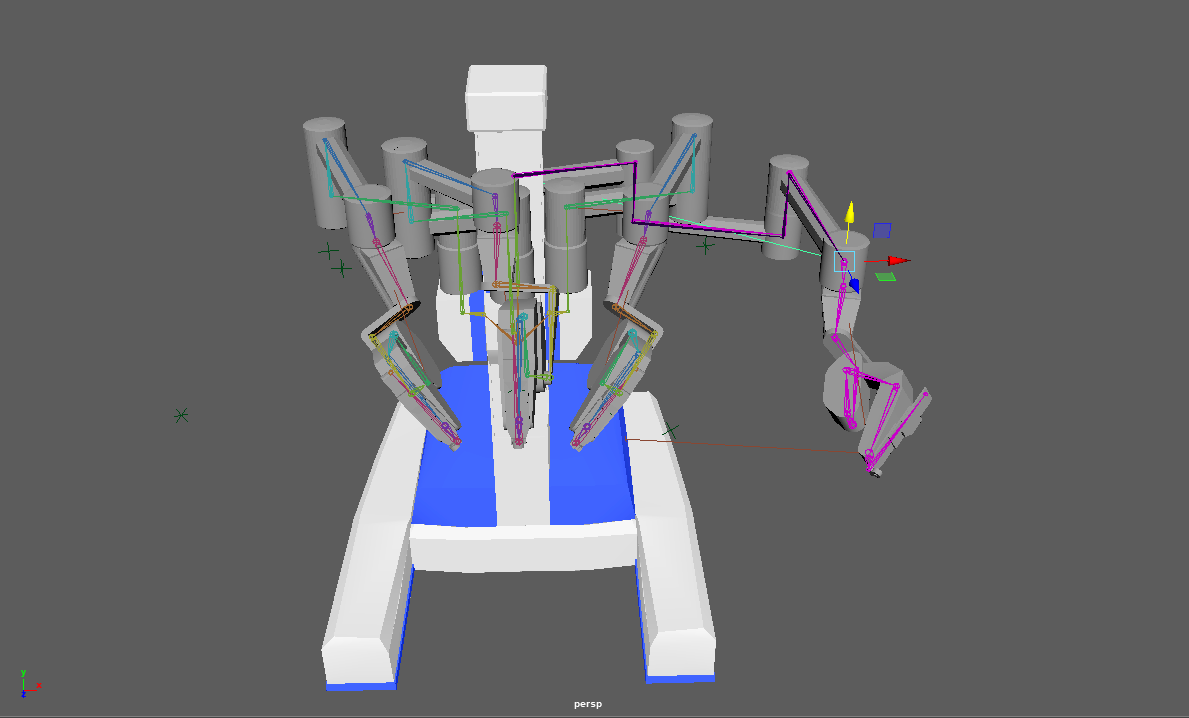
\includegraphics[width=0.3\textwidth]{ModelAnim/IK2}
	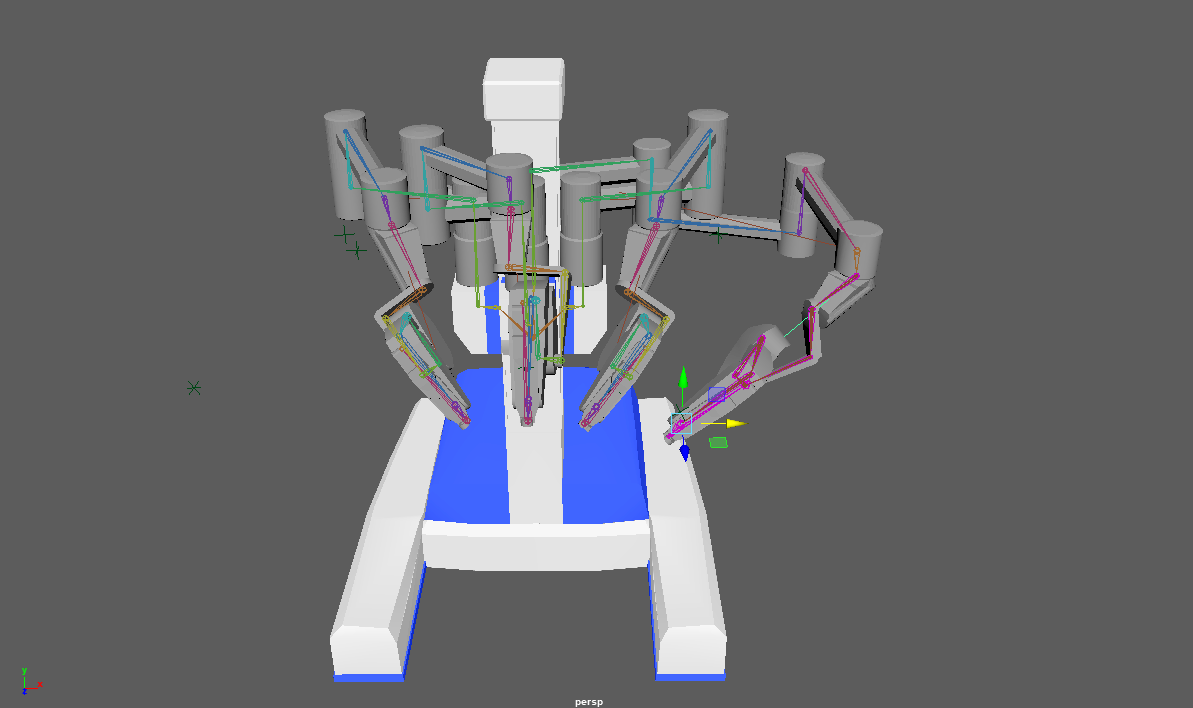
\includegraphics[width=0.3\textwidth]{ModelAnim/IK3}
	\caption{IK handles in Maya's workspace}
	\label{Fig:DoItInTheEnd}
\end{figure}

Maya has two different inverse kinematic (IK) solvers, named \textit{Single Chain IK solver} and \textit{Rotate Plane IK solver} (RP). This solution uses the RP IK solver as it's end effector only tries to reach the position of the IK handle and not the orientation. This makes the bones' rotation more reliable. This can be seen in \autoref{Fig:DoItInTheEnd}.